% ======================================================================
%  FYS4480/FYS9480  Quantum mechanics for many-particle systems
%  Week 41, October 8-9, 2026
%  Lecture slides (Beamer).  Thursday: 2 x 45 min,  Friday: 2 x 45 min.
%
%  Week 40 ended at mixed-canonical form, so this deck opens with a
%  short recap of that and then starts at matrix product operators.
%  Thursday: matrix product operators, bulk elements, fermions.
%  Friday:   the DMRG algorithm.
%  Then: the week-41 exercise set (MPS by hand, canonical forms,
%  parameter counting), the summary, the answers to the week-40 set
%  (stability matrix by Wick's theorem, positive semidefinite matrices)
%  and the outlook to week 42 (electron gas, Hartree-Fock, DFT).
%
%  Sources: chapterDMRG.tex (chapter 11 of the lecture notes), sections
%  11.3 (MPO), 11.5 (the algorithm), 11.6 (White's blocks), 11.7 (fermions).
%  Companion program: BookPrograms/chapterdmrg/dmrg.py; notebook week41.ipynb.
%
%  Build:  pdflatex week41.tex  (twice)
%  Handout (no overlays):  replace \documentclass[...] by
%           \documentclass[handout,aspectratio=169]{beamer}
% ======================================================================
\documentclass[aspectratio=169,10pt]{beamer}

% ---------------------------------------------------------------- packages
\usepackage[utf8]{inputenc}
\usepackage[T1]{fontenc}
\usepackage{amsmath,amssymb,bm,mathtools}
\usepackage{booktabs}
\usepackage[most]{tcolorbox}
\usepackage{listings}
\usepackage{hyperref}
\usepackage{tikz}
\usetikzlibrary{positioning,arrows.meta,decorations.markings,shapes.misc}
\usetikzlibrary{tikzmark}

% ---------------------------------------------------------------- look
\usetheme{default}
\useinnertheme{rectangles}
\setbeamertemplate{navigation symbols}{}
\definecolor{uioblue}{RGB}{18,52,86}
\definecolor{teal}{RGB}{0,128,128}
\definecolor{warm}{RGB}{181,73,36}
\definecolor{paleblue}{RGB}{232,240,248}
\definecolor{paleteal}{RGB}{228,244,244}
\definecolor{palewarm}{RGB}{252,238,230}
\definecolor{palegreen}{RGB}{232,244,234}
\setbeamercolor{structure}{fg=uioblue}
\setbeamercolor{title}{fg=uioblue}
\setbeamercolor{frametitle}{fg=uioblue,bg=white}
\setbeamercolor{section in toc}{fg=uioblue}
\setbeamercolor{alerted text}{fg=warm}
\setbeamercolor{block title}{fg=white,bg=uioblue}
\setbeamercolor{block body}{bg=paleblue}
\setbeamercolor{block title example}{fg=white,bg=teal}
\setbeamercolor{block body example}{bg=paleteal}
\setbeamerfont{frametitle}{size=\large,series=\bfseries}
\setbeamerfont{title}{size=\LARGE,series=\bfseries}
\setbeamertemplate{frametitle}{%
  \vspace*{0.6em}\insertframetitle\par
  \vspace*{-0.2em}{\color{teal}\rule{\textwidth}{0.6pt}}}
\setbeamertemplate{footline}{%
  \hbox{\begin{beamercolorbox}[wd=\paperwidth,ht=2.4ex,dp=1.2ex,leftskip=1em,rightskip=1em]{structure}%
  \footnotesize FYS4480/9480 -- Week 41 \hfill \insertsection \hfill \insertframenumber/\inserttotalframenumber
  \end{beamercolorbox}}}
\setbeamertemplate{itemize items}[circle]
\setbeamertemplate{enumerate items}[default]
\setbeamertemplate{section page}{%
  \begin{centering}
    {\usebeamerfont{section title}\usebeamercolor[fg]{title}\LARGE\bfseries\insertsection\par}
    \vspace{0.5em}{\color{teal}\rule{0.5\textwidth}{1pt}}
  \end{centering}}
\AtBeginSection[]{\frame{\sectionpage}}

% ---------------------------------------------------------------- boxes
\newcounter{thinkctr}
\newcommand{\thinkq}[2]{%
  \stepcounter{thinkctr}%
  \vfill
  \begin{tcolorbox}[enhanced,colback=palewarm,colframe=warm,boxrule=1.2pt,arc=4pt,
    grow to left by=6mm,grow to right by=6mm,
    left=16pt,right=16pt,top=16pt,bottom=18pt,
    fonttitle=\bfseries\Large,fontupper=\Large,
    title={Pause to think \#\thethinkctr\hfill\mdseries\normalsize(about #1 min -- discuss with your neighbour)}]
  #2
  \end{tcolorbox}
  \vfill}
\newcommand{\thinka}[1]{%
  \vfill
  \begin{tcolorbox}[enhanced,colback=paleteal,colframe=teal,boxrule=1.2pt,arc=4pt,
    grow to left by=6mm,grow to right by=6mm,
    left=16pt,right=16pt,top=16pt,bottom=18pt,
    fonttitle=\bfseries\Large,fontupper=\large,
    title={Answer to pause \#\thethinkctr}]
  #1
  \end{tcolorbox}
  \vfill}
\newcommand{\mbbox}[1]{%
  \begin{tcolorbox}[colback=paleblue,colframe=uioblue,title={\bfseries Many-body connection}]
  #1
  \end{tcolorbox}}
\newcommand{\warnbox}[1]{%
  \begin{tcolorbox}[colback=palewarm,colframe=warm,title={\bfseries A trap to avoid}]
  #1
  \end{tcolorbox}}
\newcommand{\numbox}[1]{%
  \begin{tcolorbox}[colback=palegreen,colframe=teal!70!black,title={\bfseries Measured}]
  #1
  \end{tcolorbox}}

% ---------------------------------------------------------------- code
\lstset{language=Python,basicstyle=\ttfamily\scriptsize,
  keywordstyle=\color{uioblue}\bfseries,commentstyle=\color{teal},
  stringstyle=\color{warm},showstringspaces=false,columns=fullflexible,
  frame=single,rulecolor=\color{paleblue},backgroundcolor=\color{white},
  breaklines=true}

% ---------------------------------------------------------------- macros
\newcommand{\ket}[1]{\vert #1\rangle}
\newcommand{\bra}[1]{\langle #1\vert}
\newcommand{\braket}[2]{\langle #1\vert #2\rangle}
\newcommand{\element}[3]{\langle #1\vert #2\vert #3\rangle}
\DeclareMathOperator{\tr}{tr}
\newcommand{\bigO}{\mathcal{O}}
\newcommand{\bmat}[1]{\bm{#1}}
\newcommand{\Amat}[1]{\bm{A}^{#1}}
\newcommand{\Bmat}[1]{\bm{B}^{#1}}
\newcommand{\hH}{\hat{H}}
\newcommand{\ad}[1]{a_{#1}^{\dagger}}
\newcommand{\ketbra}[2]{\vert #1\rangle\langle #2\vert}
% normal ordering with respect to the reference determinant |c> (as in week 40)
\newcommand{\nc}[1]{\bigl\{#1\bigr\}}

% ---------------------------------------------------------------- diagrams
\tikzset{
  tens/.style={draw=uioblue,fill=paleblue,thick,rounded corners=1pt,minimum size=7mm,font=\small},
  mpo/.style={draw=warm,fill=palewarm,thick,rounded corners=1pt,minimum size=7mm,font=\small},
  env/.style={draw=teal!70!black,fill=paleteal,thick,rounded corners=1pt,
              minimum width=7mm,minimum height=14mm,font=\small},
  leg/.style={thick,uioblue},
  dlab/.style={font=\scriptsize},
  every picture/.style={scale=0.8,baseline=(current bounding box.center)}
}

\graphicspath{{../BookFigures/}{./}}

% ---------------------------------------------------------------- title
\title{Matrix product operators, and finding the ground state with DMRG}
\subtitle{FYS4480/FYS9480 -- Week 41, October 8--9, 2026}
\author{Cecilie Glittum}
\institute{Department of Physics,\\
University of Oslo, Norway}
\date{}

\begin{document}

\begin{frame}[plain]
  \vspace*{0.4em}{\setbeamerfont{title}{size=\Large,series=\bfseries}\titlepage}
  \vfill
  \begin{center}\small
  Thursday: matrix product operators, what their bond dimension counts, and fermions\\
  Friday: the DMRG --- environments, the two-site update, the sweep\\[0.8em]
  {\footnotesize Reading: lecture notes chapter 11, sections 11.3 and 11.5--11.7; Schollw\"ock, Annals of Physics 326, 96 (2011), sections 4 and 6.\\
  Code: \texttt{BookPrograms/chapterdmrg/dmrg.py}; notebook \texttt{week41.ipynb}.}
  \end{center}
\end{frame}

\begin{frame}[shrink=5]{Plan for week 41}
  \begin{block}{Thursday, $2\times45$ min: matrix product operators}
    \begin{itemize}
      \item The MPO, and why its matrices are not $d\times d$
      \item Automata: Heisenberg $D=5$, pairing $D=4$ with every level coupled
      \item Where the nonzero entries sit --- and what a \emph{bulk} entry means
      \item How many channels must cross a cut: the operator Schmidt rank
      \item Fermions: Jordan--Wigner strings, and the three $\hat Z$'s of the Hubbard MPO
    \end{itemize}
  \end{block}
  \begin{block}{Friday, $2\times45$ min: the DMRG algorithm}
    \begin{itemize}
      \item Variational principle on the MPS manifold; the norm matrix $\bmat G$
      \item Environments and the effective Hamiltonian; why the cost is $\chi^3$
      \item The two-site update, and exactly how the centre moves
      \item The discarded weight as an error indicator; extrapolation
      \item Exercises: the week-41 set (MPS by hand, canonical forms, parameter counting) and answers to the week-40 set (stability matrix, positive semidefinite matrices)
    \end{itemize}
  \end{block}
\end{frame}

\begin{frame}{Where we got to last week}
  \[
    \ket\Psi=\sum_{\{s\}}\Amat{s_1}\cdots\Amat{s_{i}}\,\bm\Lambda_i\,\Bmat{s_{i+1}}\cdots\Bmat{s_L}\ket{s_1\cdots s_L}
  \]
  \begin{columns}[T]
    \column{0.5\textwidth}
    \begin{block}{What canonical form buys}
      \begin{itemize}
        \item $\sum_s\Amat{s\dagger}\Amat s=\bmat I$: left block states orthonormal
        \item $\sum_s\Bmat s\Bmat{s\dagger}=\bmat I$: right block states orthonormal
        \item $\bm\Lambda_i$ \emph{is} the Schmidt spectrum of that cut
      \end{itemize}
    \end{block}
    \column{0.5\textwidth}
    \begin{block}{So, for free}
      \begin{itemize}
        \item $\braket\Psi\Psi=\|\bm\Lambda_i\|_F^2$
        \item $S_i=-\sum_a\sigma_a^2\ln\sigma_a^2$
        \item truncation at bond $i$ is optimal
      \end{itemize}
    \end{block}
  \end{columns}
  \vspace{0.6em}
  \centering We can \alert{write} states. This week: how to write \emph{operators}, and how to \emph{find} the ground state.
\end{frame}

% ======================================================================
\section{Thursday: Matrix product operators}
% ======================================================================

\begin{frame}{Matrix product operators}
  \[
    \hH=\sum_{\{s\},\{s'\}}\bmat W^{s_1s_1'}\bmat W^{s_2s_2'}\cdots\bmat W^{s_Ls_L'}\;\ket{s_1\cdots s_L}\bra{s_1'\cdots s_L'}
  \]
  \begin{center}
  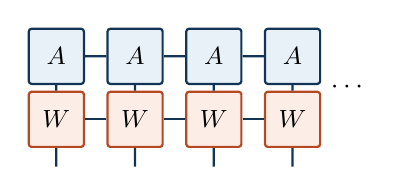
\begin{tikzpicture}[baseline]
    \foreach \i in {1,...,4}{
      \node[tens] (A\i) at (1.25*\i,1.0) {$A$};
      \node[mpo] (W\i) at (1.25*\i,0.0) {$W$};
      \draw[leg] (A\i)--(W\i); \draw[leg] (W\i)--++(0,-0.75);}
    \foreach \i [evaluate=\i as \j using int(\i+1)] in {1,...,3}{\draw[leg] (A\i)--(A\j); \draw[leg] (W\i)--(W\j);}
    \node at (1.25*4+0.9,0.5) {$\cdots$};
  \end{tikzpicture}
  \end{center}
  \begin{itemize}
    \item $\hH\ket\Psi$ is again an MPS, with bond dimension $\chi D$
    \item \emph{Automaton:} a machine walks the chain, placing operators, remembering what is open
    \item \alert{$D$ counts the partial terms open at a cut} -- not the terms in $\hH$
  \end{itemize}
\end{frame}

\begin{frame}{Why the matrices are not $d\times d$}
  Each $\bmat W_i$ has \emph{four} indices, and they do two different jobs:
  \[
    W^{s\,s'}_{\alpha\beta},\qquad
    \underbrace{s,s'=1,\dots,d}_{\text{physical: in and out}}\qquad
    \underbrace{\alpha,\beta=1,\dots,D}_{\text{bond: the automaton's state}}
  \]
  \begin{itemize}
    \item $\bmat W$ is a $D\times D$ \alert{matrix whose entries are $d\times d$ operators}
    \item The $s,s'$ are contracted with the \emph{state}; the $\alpha,\beta$ with the \emph{neighbouring $\bmat W$}
    \item $D$ has nothing to do with $d$: Heisenberg $d=2,D=5$; Hubbard $d=4,D=6$
  \end{itemize}
  \vspace{0.4em}
  \centering The automaton's memory lives on the bond index. Shape: $(D,D,d,d)$.
\end{frame}

\begin{frame}{The Heisenberg chain: $D=5$}
  \[
    \hH=J\sum_i\bm S_i\cdot\bm S_{i+1},
    \qquad
    \bmat W=\begin{pmatrix}
      \hat1 & S^x & S^y & S^z & 0\\
      0&0&0&0&JS^x\\
      0&0&0&0&JS^y\\
      0&0&0&0&JS^z\\
      0&0&0&0&\hat1
    \end{pmatrix}
  \]
  \centering First site: the first row. Last site: the last column.
  \begin{itemize}
    \item The five states: nothing placed; $S^x$, $S^y$ or $S^z$ waiting; finished
    \item Each path $1\to\alpha\to5$ places exactly one bond term
    \item An $L=100$ chain has $297$ terms and still $D=5$
  \end{itemize}
\end{frame}

\begin{frame}{Pause to think: what the bond dimension counts}
  \thinkq{4}{
  \begin{enumerate}
    \item An $L=100$ Heisenberg chain has $297$ terms, and $D=5$. Explain the discrepancy in one sentence.
    \item What is $D$ for $J_1\sum_i\bm S_i\cdot\bm S_{i+1}+J_2\sum_i\bm S_i\cdot\bm S_{i+2}$?
  \end{enumerate}}
\end{frame}

\begin{frame}{Answer}
  \thinka{
  \begin{enumerate}
    \item $D$ counts terms open \emph{at one cut}, and at most one bond term straddles a cut; the $297$ terms are \emph{paths} through the network, not its width.
    \item $D=8$: each component now needs two waiting states, $1+3+3+1$.
  \end{enumerate}}
\end{frame}

\begin{frame}{Where do the nonzero entries sit?}
  \begin{center}\small
  \begin{tabular}{@{}lll@{}}\toprule
  region of $\bmat W$ & transition & meaning\\\midrule
  first row, $W_{1\beta}$ & idle $\to\beta$ & \alert{start} a term at this site\\
  last column, $W_{\alpha D}$ & $\alpha\to$ done & \alert{finish} a term at this site\\
  bulk, $W_{\alpha\beta}$, $1<\alpha,\beta<D$ & $\alpha\to\beta$ & \alert{carry} a half-finished term across this site\\\bottomrule
  \end{tabular}
  \end{center}
  \vspace{0.5em}
  \begin{itemize}
    \item Nearest neighbour: the machine waits exactly \emph{one} step, so the bulk is \emph{empty}
    \item \alert{Bulk entries are memory} -- they appear when something must be remembered longer
  \end{itemize}
\end{frame}

\begin{frame}{Three bulk entries, three kinds of long range}
  \begin{columns}[T]
    \column{0.34\textwidth}
    \begin{block}{Range 2}
      \[\bmat W=\begin{pmatrix}\hat1&\hat o&0&0\\0&0&\alert{\hat1}&0\\0&0&0&\hat o\\0&0&0&\hat1\end{pmatrix}\]
      \centering $D=r+2$ at range $r$
    \end{block}
    \column{0.32\textwidth}
    \begin{block}{Exponential}
      \[\bmat W=\begin{pmatrix}\hat1&\hat o&0\\0&\alert{\lambda\hat1}&\lambda\hat o\\0&0&\hat1\end{pmatrix}\]
      \centering $\sum_{i<j}\lambda^{j-i}\hat o_i\hat o_j$, $D=3$ at \emph{any} range
    \end{block}
    \column{0.32\textwidth}
    \begin{block}{$\lambda(\hat N-N_0)^2$}
      Same automaton, \alert{no decay at all}:
      \[\bmat W=\begin{pmatrix}\hat1&\hat n&\ast\\0&\alert{\hat1}&2\lambda\hat n\\0&0&\hat1\end{pmatrix}\]
      \centering\scriptsize $\ast=\lambda(1-2N_0)\,\hat n+\dfrac{\lambda N_0^2}{L}\,\hat1$\\[3pt]
      $\bigO(L^2)$ terms, \alert{one bit} of memory.
    \end{block}
  \end{columns}
  \vspace{0.5em}
A self-loop sums a geometric series for free. Added to an existing MPO, the penalty costs \alert{one} extra state.\\[2pt]
  {\scriptsize $\hat o$ is any Hermitian one-site operator; $\hat n=\hat a^\dagger\hat a=\mathrm{diag}(0,1)$ is the
  \emph{local} occupation, $\hat N=\sum_p\hat n_p$ the \emph{global} one, and $N_0$ a plain number.\\
  Two different $\lambda$'s: a \emph{decay factor} in the middle column, a \emph{strength} in the right one.}
\end{frame}

\begin{frame}{How many channels must cross a cut?}
  Split $\hH$ at a bond: $\;\hH=\hH_A\otimes\hat1+\hat1\otimes\hH_B+\sum_k\hat X_k\otimes\hat Y_k$, and count.
  \[
    D_{\min}=\text{\alert{operator Schmidt rank}}
    \qquad\text{(the SVD of $\hH$, with $\langle\hat X,\hat Y\rangle=\tr(\hat X^\dagger\hat Y)$)}
  \]
  \begin{center}\small
  \begin{tabular}{@{}lccccc@{}}\toprule
   & \multicolumn{5}{c}{rank at each cut}\\\midrule
  Heisenberg, open ($L=6$) & 4&5&5&5&4\\
  Heisenberg, \alert{ring} ($L=6$) & 4&8&8&8&4\\
  pairing, open ($L=4$) & 4&4&4&&\\\bottomrule
  \end{tabular}
  \end{center}
  \begin{itemize}
    \item A ring cuts \emph{two} bonds: $1+1+3+3=8$. The operator is the cheap part --- $\chi$ roughly \alert{squares}
    \item The automaton gives \emph{a} valid $D$; only the rank gives \emph{the} smallest
  \end{itemize}
\end{frame}

\begin{frame}{The staircase shape is a gauge, not a property of $\hH$}
  \[
    \bmat W^{[i]}\ \longrightarrow\ \bmat X_{i-1}^{-1}\bmat W^{[i]}\bmat X_i
    \qquad\text{leaves $\hH$ and $D$ unchanged}
  \]
  \begin{columns}[T]
    \column{0.42\textwidth}
    \numbox{Random $\bmat X$ on the $D=5$ Heisenberg MPO: all $25$ blocks become nonzero, and
    $\max|\Delta\hH|=1.2\times10^{-14}$.}
    \column{0.54\textwidth}
    \begin{itemize}
      \item The readable upper-triangular form is the \emph{automaton gauge}
      \item An SVD-compressed MPO is normally \alert{dense} --- not a bug
      \item The \emph{sparsity pattern} is gauge-dependent; $\hH$ itself, $D$ and the operator-Schmidt data are not
    \end{itemize}
  \end{columns}
\end{frame}

\begin{frame}{Fermions on a chain: Jordan--Wigner}
  \[
    \ad m=\Bigl(\prod_{k<m}\hat Z_k\Bigr)\hat\sigma^+_m
    \qquad\Longrightarrow\qquad
    \ad i\hat a_j=\hat\sigma^+_i\,\underbrace{\hat Z_{i+1}\cdots\hat Z_{j-1}}_{\text{the string}}\,\hat\sigma^-_j
  \]
  \centering The string runs over the orbitals \alert{strictly between} $i$ and $j$.
  \begin{itemize}
    \item Nearest neighbours: \emph{no string at all}, $\ad i\hat a_{i+1}=\hat\sigma^+_i\hat\sigma^-_{i+1}$
    \item Pairing: strings \alert{cancel} -- $\hat P^\pm_p$ is \emph{even}, both operators on one site
    \item Strings cost \emph{no} bond dimension. They cost \alert{locality}: on a ring or in 2D, length $\bigO(L)$
  \end{itemize}
  \vspace{0.3em}
  \warnbox{Test a fermionic MPO at range \emph{two}, never at range one: at range one there is no intermediate site, so writing $\hat 1$ for $\hat Z$ cannot show. At $r=2$ it is off by $\max|\Delta\hH|=2t$.}
\end{frame}

\begin{frame}{The Hubbard MPO: three different $\hat Z$'s}
  \begin{center}\small
  \begin{tabular}{@{}llp{6.0cm}@{}}\toprule
   & where & what it does\\\midrule
  (i) within-site & inside $\hat c^\dagger_\downarrow=\hat Z\otimes\hat\sigma^+$ & the down operator passes the up orbital of its \emph{own} site\\
  (ii) between-site & on other sites' orbitals & the genuine Jordan--Wigner string\\
  (iii) $\hat F=\hat Z\otimes\hat Z$ & a cell of $\bmat W$ & parity of a \emph{whole} site -- what the automaton carries\\\bottomrule
  \end{tabular}
  \end{center}
  \begin{center}\small
  \begin{tabular}{@{}l|cc|cc|l@{}}\toprule
  orbital: & $1\!\uparrow$ & $1\!\downarrow$ & $2\!\uparrow$ & $2\!\downarrow$ & \\
   & \multicolumn{2}{c|}{\emph{site 1}} & \multicolumn{2}{c|}{\emph{site 2}} & \\\midrule
  $\hat c^\dagger_{1\uparrow}\hat c_{2\uparrow}$ & $\hat\sigma^+$ & \alert{$\hat Z$} & $\hat\sigma^-$ & & string \alert{inside site 1}\\
  $\hat c^\dagger_{1\downarrow}\hat c_{2\downarrow}$ & & $\hat\sigma^+$ & \alert{$\hat Z$} & $\hat\sigma^-$ & string \alert{inside site 2}\\\bottomrule
  \end{tabular}
  \end{center}
  \centering The up hop jumps over its \emph{own} site's down orbital; the down hop over the \emph{next} site's up orbital.
\end{frame}

\begin{frame}{One rule for both spins, and what $\hat F$ is really doing}
  \[
    \hat c^\dagger_{i\sigma}\hat c_{i+1,\sigma}=\bigl(\hat c^\dagger_\sigma\hat F\bigr)_i\otimes\bigl(\hat c_\sigma\bigr)_{i+1}
  \]
  \[
    \underbrace{\hat c^\dagger_\uparrow\hat F=\hat\sigma^+\!\otimes\hat Z}_{\hat F\ \textbf{adds}\ \text{the }\hat Z}
    \qquad\qquad
    \underbrace{\hat c^\dagger_\downarrow\hat F=\hat 1\otimes\hat\sigma^+}_{\hat F\ \textbf{cancels}\ \text{the }\hat Z}
  \]
  \begin{itemize}
    \item For $\downarrow$, the within-site $\hat Z$ was the parity of the \emph{same} site's up orbital --- not between the two operators, so it must go
    \item The $\hat Z$ the down hop \emph{does} need reappears on the right, inside $\hat c_\downarrow=\hat Z\otimes\hat\sigma^-$
    \item Hubbard: $D=6$ (ring: $10$). Verified against bare fermions, $\max|\Delta\hH|=0$
  \end{itemize}
  \warnbox{The h.c.\ channel is $(\hat F\hat c_\sigma)_i\otimes(\hat c^\dagger_\sigma)_{i+1}$, \emph{not} $\hat c_\sigma\hat F$: $\{\hat c,\hat F\}=0$. Writing it the wrong way gives $\max|\Delta\hH|=2t$ \alert{and exactly the right ground-state energy}. A correct energy is \textit{not} a test of an MPO.}
\end{frame}

\begin{frame}{Bond dimensions to know}

    \begin{block}{From the automaton}
      \begin{itemize}
        \item Ising $D=3$; Heisenberg $D=5$
        \item Pairing $D=4$; $+\lambda(\hat N-N_0)^2$: $D=5$
        \item Hubbard chain $D=6$ (ring $10$)
        \item Particle--hole term $D=14$
        \item Range-$r$ hopping, spinless: $D=2r+2$
      \end{itemize}
    \end{block}
\end{frame}

% ======================================================================
\section{Friday: The DMRG algorithm}
% ======================================================================

\begin{frame}{The variational principle, on a new manifold}
  \[
    E[\Psi]=\frac{\element{\Psi}{\hH}{\Psi}}{\braket\Psi\Psi}
    \qquad\text{minimised over MPS with bond dimension}\le\chi
  \]
  \begin{itemize}
    \item The trial space is no longer a set of determinants: it is \alert{states with bounded entanglement}
    \item An MPS is a \emph{product}, so with all but one tensor frozen it is \alert{linear} in the last one
    \item So each local problem is an ordinary eigenproblem --- and we \alert{sweep}
  \end{itemize}
  \vspace{0.4em}
  \mbbox{Exactly the structure of the self-consistent field: a hard non-linear problem solved by iterating easy linear ones. The difference: each local step minimises over its subspace --- exactly in the ideal algorithm, in practice up to
  the eigensolver tolerance.}
\end{frame}

\begin{frame}{Being variational has a price: the norm matrix $\bmat G$}
  We want a \alert{variational} method, so we minimise a \emph{ratio} --- and the denominator is where $\bmat G$ is born.
  With everything frozen except $\bm\Theta$, write $\ket\Psi=\sum_\alpha\Theta_\alpha\ket{\phi_\alpha}$:
  \[
    E=\frac{\element\Psi\hH\Psi}{\braket\Psi\Psi}
     =\frac{\bm\Theta^\dagger\hH_{\rm eff}\bm\Theta}{\bm\Theta^\dagger\bmat G\bm\Theta},
    \qquad
    \bmat G_{\alpha\beta}=\braket{\phi_\alpha}{\phi_\beta}
  \]
  \begin{itemize}
    \item In an \alert{orthonormal} basis, $\braket vw=\sum_i v_i^*w_i$. In \emph{any other} basis a matrix sits in the middle: $\braket vw=\sum_{ij}v_i^*\bmat G_{ij}w_j$
    \item So $\bmat G$ is just the table of inner products of the basis you happened to use --- and $\bmat G=\bmat I$ \emph{means} that basis is orthonormal
    \item Minimising $\dfrac{\bm x^\dagger\bmat A\bm x}{\bm x^\dagger\bm x}$ gives $\bmat A\bm x=\lambda\bm x$; minimising $\dfrac{\bm x^\dagger\bmat A\bm x}{\bm x^\dagger\bmat G\bm x}$ gives $\bmat A\bm x=\lambda\bmat G\bm x$ --- the $\bmat H\bmat c=E\bmat S\bmat c$ of Section 1.15
    \item Canonical form makes the block states orthonormal $\Rightarrow$ $\bmat G=\bmat I$, an \alert{ordinary} eigenproblem again
  \end{itemize}
\end{frame}

\begin{frame}{Why that matters in practice}
  \numbox{Random $L=6$, $\chi=4$ MPS: $\mathrm{cond}(\bmat G)=9.0\times10^{9}$. \emph{The same state}, canonicalised:
  $\mathrm{cond}(\bmat G)=1$ and $\max|\bmat G-\bmat I|=3.3\times10^{-16}$. Nothing physical changed --- only the gauge.}
  \begin{itemize}
    \item A generalised solver must factorise or solve with $\bmat G$ --- \alert{never form $\bmat G^{-1}$} --- and
          ill-conditioning amplifies rounding noise by $\mathrm{cond}(\bmat G)$
    \item The gauge freedom $\Amat s\to\Amat s\bmat X$ lets block states become nearly \emph{parallel}. Make two agree to one part in $10^6$: $\mathrm{cond}(\bmat G)=1.4\times10^{16}$ --- numerically singular
    \item \alert{A redundant bond dimension is not just wasteful, it is ill-conditioned}
  \end{itemize}
  \vspace{0.3em}
  \centering\small Section 1.13 warns about exactly this for near-linearly-dependent basis sets.
  There the cure costs a diagonalisation; here it costs a QR.
\end{frame}

\begin{frame}{Environments: freeze everything but two sites}
  \[
    \element{\Psi}{\hH}{\Psi}=\sum\Theta^*_{astb}\,L_{a b_L a'}W^{ss'}_{b_Lc}W^{tt'}_{c b_R}R_{b b_R b'}\,\Theta_{a's't'b'}
  \]
  \begin{center}
  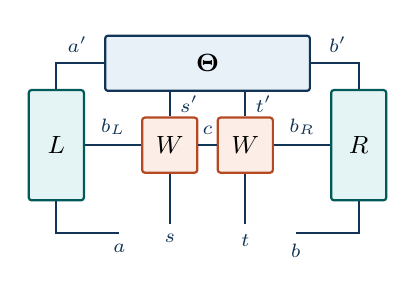
\begin{tikzpicture}[x=1cm,y=1cm,baseline]
    \node[tens,minimum width=26mm] (T) at (2.4,1.7) {$\bm\Theta$};
    \node[env] (L) at (0,0.4) {$L$};
    \node[env] (R) at (4.8,0.4) {$R$};
    \node[mpo] (W1) at (1.8,0.4) {$W$};
    \node[mpo] (W2) at (3.0,0.4) {$W$};
    \draw[leg] (L.north) |- (T.west) node[dlab,pos=0.72,above] {$a'$};
    \draw[leg] (R.north) |- (T.east) node[dlab,pos=0.72,above] {$b'$};
    \draw[leg] (T.south -| W1) -- (W1.north) node[dlab,midway,right] {$s'$};
    \draw[leg] (T.south -| W2) -- (W2.north) node[dlab,midway,right] {$t'$};
    \draw[leg] (L.east) -- (W1.west) node[dlab,midway,above] {$b_L$};
    \draw[leg] (W1.east) -- (W2.west) node[dlab,midway,above] {$c$};
    \draw[leg] (W2.east) -- (R.west) node[dlab,midway,above] {$b_R$};
    \draw[leg] (L.south) |- (1.0,-1.0) node[dlab,below] {$a$};
    \draw[leg] (R.south) |- (3.8,-1.0) node[dlab,below] {$b$};
    \draw[leg] (W1.south) -- ++(0,-0.8) node[dlab,below] {$s$};
    \draw[leg] (W2.south) -- ++(0,-0.8) node[dlab,below] {$t$};
  \end{tikzpicture}
  \end{center}
  \centering\small
  \alert{Why three indices?} A cut severs exactly three lines: one in the bra, one in the MPO, one in the ket. So $L,R$ are $\chi\times D\times\chi$.
\end{frame}

\begin{frame}{Reading that diagram}
  \begin{itemize}
    \item It is $\hH_{\rm eff}\bm\Theta$, \emph{not} $\element\Psi\hH\Psi$: the bra $\bm\Theta^*$ has been removed
    \item \alert{Primed} indices $a',s',t',b'$ are summed against the input; the four \alert{unprimed} legs dangle --- they are the result
    \item Four legs in, four legs out, same shape $(\chi,d,d,\chi)$: that \emph{is} ``a linear map on the space $\bm\Theta$ lives in''
    \item $\bm\Theta$ is \alert{one} box with \emph{no internal bond}. The bond is created later, by the SVD
  \end{itemize}
  \vspace{0.4em}
  \begin{block}{Never form $\hH_{\rm eff}$ as a matrix}
    Lanczos needs only the \emph{action}: four contractions, $\bigO(\chi^3d^2D+\chi^2d^3D^2)$.
    At $\chi=64$, $d=4$ the matrix would be $65\,536\times65\,536$.
  \end{block}
\end{frame}

\begin{frame}{Why $\chi^3$}
  \[
    \sum_{a'}L_{a\,b\,a'}\,\Theta_{a'\,s_1s_2\,b_r}
    \qquad\Longrightarrow\qquad
    \boxed{\;\text{two free bond legs}\times\text{one summed bond leg}=\chi^3\;}
  \]
  \begin{itemize}
    \item Every object carries at most \emph{two} bond legs: $\bm\Theta$ is $(\chi,d,d,\chi)$, $L$ and $R$ are $(\chi,D,\chi)$
    \item The result keeps $\chi^2$ entries, each costing a sum over $\chi$ terms
    \item This is just the cost of multiplying two $\chi\times\chi$ matrices --- and that is every step
    \item Form an intermediate with \alert{three} bond legs and you pay $\chi^4$
  \end{itemize}
\end{frame}

\begin{frame}{The two-site update}
  \begin{enumerate}
    \item \textbf{Form $\bm\Theta$} from the two central tensors. \emph{The shared bond disappears, so the SVD may give it a new dimension --- up to $\chi d$, not unlimited}
    \item \textbf{Solve} $\hH_{\rm eff}\bm\Theta=E\bm\Theta$ by Lanczos, matrix-free, from the current $\bm\Theta$. \emph{The only place physics enters}
    \item \textbf{Reshape and SVD}: $\bm\Theta_{(as),(tb)}=\bmat U\bm\Sigma\bmat V^\dagger$. \emph{This \alert{is} the Schmidt decomposition of that bond}
    \item \textbf{Truncate} to $\chi$; record $\varepsilon_\chi=\sum_{k>\chi}\sigma_k^2$. \emph{Optimal, by Eckart--Young}
    \item \textbf{Move the centre} and extend the environment
  \end{enumerate}
  \vspace{0.3em}
  \centering Do not \emph{over}converge Lanczos in the early sweeps --- the tensor is recomputed next sweep anyway ---
  and tighten its tolerance near convergence. Converge the \alert{sweep}, not the step.
\end{frame}

\begin{frame}{How the centre actually moves}
  \centering You never move $\bm\Theta$. You \alert{split} it and keep one half.
  \[
    \Theta_{astb}=\sum_c(\bmat M_i)_{asc}(\Bmat{}_{i+1})_{ctb}
    \ \xrightarrow{\ \rm SVD\ }\
    (\Amat{}_i)_{asc}=U_{(as),c},\quad
    (\bmat M_{i+1})_{ctb}=(\bm\Sigma\bmat V^\dagger)_{c,(tb)}
  \]
  \[
    \text{next step:}\qquad
    \Theta'_{ctub'}=\sum_b(\bmat M_{i+1})_{ctb}\,(\Bmat{}_{i+2})_{bub'}
  \]
  \begin{center}\small
  \begin{tabular}{@{}llll@{}}\toprule
  direction & site $i$ & site $i+1$ & extend\\\midrule
  \textbf{right} & $\Amat{}_i=\bmat U$ (left-can.) & $\bmat M_{i+1}=\bm\Sigma\bmat V^\dagger$ (centre) & $L_{i+1}$\\
  \textbf{left} & $\bmat M_i=\bmat U\bm\Sigma$ (centre) & $\Bmat{}_{i+1}=\bmat V^\dagger$ (right-can.) & $R_{i+1}$\\\bottomrule
  \end{tabular}
  \end{center}
  \centering\small $\bm\Sigma$ always stays with the centre --- it is the part that is \emph{not} canonical.
\end{frame}

\begin{frame}{One sweep, watched: there \emph{and} back}
  \begin{columns}[T]
    \column{0.49\textwidth}
    \begin{center}\scriptsize\ttfamily
    \begin{tabular}{@{}ll@{}}\toprule
    moving right & 1 2 3 4 5 6\\\midrule
    start (all right-canonical) & R R R R R R\\
    bond (1,2) & L C R R R R\\
    bond (2,3) & L L C R R R\\
    bond (3,4) & L L L C R R\\
    bond (4,5) & L L L L C R\\
    bond (5,6) & L L L L L L\\\bottomrule
    \end{tabular}
    \end{center}
    \column{0.49\textwidth}
    \begin{center}\scriptsize\ttfamily
    \begin{tabular}{@{}ll@{}}\toprule
    then back & 1 2 3 4 5 6\\\midrule
    bond (5,6) & L L L L C R\\
    bond (4,5) & L L L C R R\\
    bond (3,4) & L L C R R R\\
    bond (2,3) & L C R R R R\\
    bond (1,2) & R R R R R R\\
    \multicolumn{2}{@{}l@{}}{\rm\itshape ready for the next sweep}\\\bottomrule
    \end{tabular}
    \end{center}
  \end{columns}
  \normalfont
  \vspace{0.2em}
  \small
  \begin{itemize}
    \item \texttt{C} marches one site per step; an \texttt{L} wall grows behind it, the \texttt{R} wall retreats in front
    \item \alert{One sweep is the round trip}: the return pass revisits every bond now that the \emph{opposite}
          environment has moved. Canonical form, and so $\bmat G=\bmat I$, holds in either direction
    \item At the turn \texttt{(5,6)} is solved twice with \emph{identical} environments, so an exact solve returns the
          \emph{same state} (measured: overlap $1.000000000000$, $\Delta E=0$) --- a \alert{gauge move}, not an
          improvement. Hence $2(L-1)$ local solves with this convention, $2L-3$ if you skip it
    \item Beware: many papers call one \emph{pass} a sweep, and the round trip two --- a factor of two in
          ``converged after 5 sweeps''
  \end{itemize}
\end{frame}

\begin{frame}{Pause to think: one site or two?}
  \thinkq{4}{
  \begin{enumerate}
    \item A one-site update optimises $\bmat M_i$ alone, then moves on. Why can it \emph{never} increase the bond dimension?
    \item The two-site $\bm\Theta$ is $\chi d\times d\chi$. What does its SVD let you do that the one-site version cannot?
    \item What do you pay for it?
  \end{enumerate}}
\end{frame}

\begin{frame}{Answer}
  \thinka{
  \begin{enumerate}
    \item The local eigenproblem lives in the space the \emph{current} bonds already span. It re-mixes those $\chi$ states; it cannot invent new ones --- and it is stuck in the symmetry sector it started in.
    \item Its SVD has up to $\chi d$ singular values, so it can \alert{grow} $\chi$ exactly where the state needs it.
    \item A factor $d$ in cost, and a truncation at \emph{every} step.
  \end{enumerate}}
\end{frame}

\begin{frame}{Single-site DMRG: the objection, and why it is not the whole story}
  The answer above is the classic objection --- and it applies to the \emph{plain} single-site update.
  With a \alert{subspace expansion} it does not, and production codes often prefer single-site.
  \small
  \begin{columns}[T]
    \column{0.49\textwidth}
    \begin{block}{In favour of single-site}
      \begin{itemize}
        \item Cheaper: no factor $d$ from the two-site tensor, smaller SVD
        \item \alert{No truncation step at all} --- so the energy is \emph{strictly} monotone
        \item Symmetry quantum numbers on the bond preserved exactly
        \item \alert{With the expansion it can converge faster than two-site} while avoiding the same
              local-minimum traps: the expansion is \emph{Hamiltonian-informed}
      \end{itemize}
    \end{block}
    \column{0.49\textwidth}
    \begin{block}{Against}
      \begin{itemize}
        \item Plain version cannot grow $\chi$, and sticks in its symmetry sector
        \item DMRG3S-type fixes need a mixing parameter $\alpha$, annealed to zero (newer controlled bond
              expansion does not)
        \item No $\varepsilon_\chi$ for free --- the error indicator must come from elsewhere
      \end{itemize}
    \end{block}
  \end{columns}
\end{frame}

\begin{frame}{The mixer, and which to use}
  The cure for getting stuck is the \alert{mixer} --- a \emph{subspace expansion} that perturbs the SVD so that the
  retained Schmidt states include directions the current state does not occupy yet.
  \begin{tcolorbox}[colback=paleteal,colframe=teal,title={\bfseries In practice},
      fonttitle=\bfseries\small,boxsep=2pt,left=6pt,right=6pt,top=3pt,bottom=3pt]
    \small Single-site stays \emph{by construction in the subspace of a given bond-dimension MPS, unless you use a
    mixer} --- so always run one. Two-site \emph{formally avoids this problem} but can still get stuck: keep the mixer on for the \emph{initial} sweeps, then switch it off to converge.
  \end{tcolorbox}
  \begin{itemize}
    \item So the ranking is: plain single-site \emph{worst}; two-site safe in principle; single-site $+$ expansion can be \emph{best}
    \item With conserved quantum numbers two-site \emph{can} create new sectors on the central bond --- but not ones
          excluded by the \alert{outer} bond spaces, and expansion helps when those are deficient
  \end{itemize}
  \vspace{0.2em}
  \centering\scriptsize White (2005); Hubig, McCulloch \& Schollw\"ock (2015), ``strictly single-site'' DMRG3S.\\[2pt]
  \normalsize\alert{With two-site, the SVD makes the truncation --- and its error indicator --- visible.}
\end{frame}

\begin{frame}{The discarded weight is an error \emph{indicator}}
  Write $\ket{\psi_\chi}=\ket\psi+\ket\delta$ with $\braket\delta\delta=\varepsilon_\chi$. Since $\ket\psi$ is stationary, the first-order term vanishes:
  \[
    E(\chi)-E_0=\element{\delta}{(\hH-E_0)}{\delta}
    =\varepsilon_\chi\cdot\underbrace{\frac{\element{\delta}{(\hH-E_0)}{\delta}}{\braket\delta\delta}}_{\textstyle\langle\Delta E\rangle}
  \]
  \begin{itemize}
    \item The constant of proportionality is \alert{an energy}: the mean excitation energy of what you threw away
    \item Second order in the state error, and always \alert{positive} --- variational
  \end{itemize}
  \warnbox{\small But $\varepsilon_\chi$ is the weight discarded at \emph{one local SVD}, not $\|\delta\|^2$ against the
  exact ground state. The near-linear law is an empirical small-$\varepsilon$ rule, \alert{not a rigorous bound}, and
  other observables can be off by much more.}
  \centering\alert{Run at several $\chi$, plot $E$ against $\varepsilon_\chi$, extrapolate to $\varepsilon=0$.}
\end{frame}

\begin{frame}{What the numbers look like}
  \begin{center}\small
  \begin{tabular}{@{}lllll@{}}\toprule
  $\chi$ & $E_{\rm DMRG}$ & $E-E_0$ & $\varepsilon_\chi$ & $S_{L/2}$\\\midrule
  4 & 2.2435302961 & $4.1\times10^{-1}$ & $9.1\times10^{-3}$ & 1.0114\\
  8 & 1.8655652393 & $3.6\times10^{-2}$ & $1.2\times10^{-3}$ & 1.0898\\
  16 & 1.8326023377 & $3.5\times10^{-3}$ & $1.3\times10^{-4}$ & 1.1064\\
  32 & 1.8291612166 & $5.5\times10^{-5}$ & $2.4\times10^{-6}$ & 1.1084\\
  64 & 1.8291067166 & $4.5\times10^{-8}$ & $2.2\times10^{-9}$ & 1.1084\\
  exact & 1.8291066715 &&&\\\bottomrule
  \end{tabular}
  \end{center}
  \centering\small pairing $+$ particle--hole, $L=N=8$, $g=1$, $f=0.5$. \quad
  $\varepsilon_\chi$ here is the \alert{maximum over bonds} in the last sweep --- conventions differ, so say which you use.
  \begin{itemize}
    \item $\Delta E/\varepsilon_\chi$ drifts from $46$ to $21$ --- \alert{those numbers are energies}
    \item A line through the three \emph{most accurate} runs lands within $5\times10^{-6}$; through the three cheapest, it misses by $10^{-2}$
  \end{itemize}
\end{frame}

\begin{frame}{Does the energy really fall monotonically?}
  Each update is \emph{two} steps with opposite characters:
  \begin{columns}[T]
    \column{0.48\textwidth}
    \begin{block}{The eigensolve: cannot increase $E$}
      An exact minimisation over a subspace that \emph{contains the current state}.
    \end{block}
    \column{0.48\textwidth}
    \warnbox{The truncation: \emph{can}. Throwing away $\varepsilon_\chi$ moves the state and raises $E$ by $\bigO(\varepsilon_\chi)$.}
  \end{columns}
  \vspace{0.4em}
  \begin{itemize}
    \item Monotonicity is \alert{not a theorem} --- it is what happens once $\varepsilon_\chi$ is small
    \item Early on, with $\chi$ still growing, the energy can tick \emph{upwards}. Not a bug
    \item What \emph{is} guaranteed: every printed energy is an \alert{upper bound} on $E_0$
  \end{itemize}
\end{frame}

\begin{frame}{How do you know it has converged?}
  Four things, all at once --- and checking only the first is the commonest mistake:
  \begin{enumerate}
    \item the energy has stopped changing between sweeps
    \item $\varepsilon_\chi$ is small \alert{and falls when you raise $\chi$} --- flat energy $+$ large
          $\varepsilon_\chi$ means \alert{not demonstrably converged}: either stuck, or $\chi$ simply too small
    \item $\langle\hat N\rangle$ is the value you asked for
    \item $S_{L/2}$ has stopped growing with $\chi$
  \end{enumerate}
  \vspace{0.4em}
  \numbox{How worried about local minima? For \emph{these} models, not very: $L=20$ Heisenberg from eight random starts agrees to $5\times10^{-14}$ at $\chi=4$. If your energies move with the seed, suspect a \alert{bug} before suspecting physics. Genuine local minima live in frustration, all-to-all couplings and chemistry.}
\end{frame}

\begin{frame}{A 200-line NumPy code, Heisenberg at $L=32$}
  \begin{center}\small
  \begin{tabular}{@{}rrrrr@{}}\toprule
  $\chi$ & $E_{\rm DMRG}$ & $\varepsilon_\chi$ & $S_{L/2}$ & time\\\midrule
  8 & $-13.995308101464$ & $4.0\times10^{-5}$ & 0.6941 & 0.3\,s\\
  16 & $-13.997257888143$ & $3.1\times10^{-6}$ & 0.7203 & 0.5\,s\\
  32 & $-13.997315266845$ & $1.2\times10^{-8}$ & 0.7215 & 0.9\,s\\
  64 & $-13.997315618007$ & $6.9\times10^{-12}$ & 0.7215 & 2.1\,s\\\bottomrule
  \end{tabular}
  \end{center}
  \begin{itemize}
    \item Energy falls monotonically, by one to two orders per doubling of $\chi$
    \item $S_{L/2}$ has converged by $\chi=32$ --- which is why the last row buys so little
    \item Dense diagonalisation in the full $2^{32}$ basis is impractical; this takes two seconds
  \end{itemize}
  \centering\alert{Report $\varepsilon_\chi$ as well as $\chi$} --- and the sweep schedule and tolerances.
\end{frame}

\begin{frame}{Where the name comes from: White, 1992}
  \begin{itemize}
    \item Grow a block site by site; its space grows as $d^\ell$, so truncate to $\chi$ states. \alert{Which $\chi$?}
    \item Wilson's NRG kept the lowest eigenstates of the \emph{block} Hamiltonian --- wrong once the block is embedded
    \item White: form the \emph{superblock}, get its ground state, trace out the environment, keep the largest eigenvectors of $\rho_A$
  \end{itemize}
  \vspace{0.4em}
  \begin{block}{That is exactly our Schmidt truncation}
    The eigenvectors of $\rho_A$ are the Schmidt states; its eigenvalues are $\sigma_k^2$; keeping the largest minimises the discarded weight. ``Density matrix'' $=$ the reduced density matrix of the cut; ``renormalisation group'' $=$ the block growing.
  \end{block}
  \centering\small \emph{Infinite-system} algorithm: grow to length $L$. \emph{Finite-system} algorithm: then sweep --- what we described.
\end{frame}

% ======================================================================
\section{Exercise session}
% ======================================================================

\begin{frame}{Exercise 1: an MPS for the W state}
  \[
    \ket{W}=\tfrac1{\sqrt3}\bigl(\ket{100}+\ket{010}+\ket{001}\bigr)
  \]
  \begin{enumerate}
    \item Write the coefficient matrix for the cut after site 1 and find its rank. What is $\chi_1$? Same for $\chi_2$.
    \item Construct $\Amat{s}_i$ explicitly. \emph{Hint:} let the bond index record one bit --- \alert{has the excitation been placed yet?}
    \item Check that $C_{100}=C_{010}=C_{001}=1/\sqrt3$. Why does $C_{110}=0$ come out automatically?
    \item Generalise to $L$ sites. Does $\chi$ grow with $L$?
    \item Compare with GHZ, $\tfrac1{\sqrt2}(\ket{0\cdots0}+\ket{1\cdots1})$, which also has $\chi=2$. In each case, \emph{what does the bond index remember}?
  \end{enumerate}
\end{frame}

\begin{frame}{Exercise 2(a): right- and mixed-canonical form}
  In the lectures of Week 40, we built the left-canonical MPS by $L-1$ SVDs sweeping \emph{rightwards}. Now do it the other way.
  \begin{enumerate}
    \item Repeat the construction starting from the \emph{right} end. Show that the tensors you get satisfy
      \[\sum_s\Bmat s\Bmat{s\dagger}=\bmat I\]
      and that this makes the \emph{right} block states orthonormal.
    \item Now stop halfway: sweep in from the left to site $i$ and in from the right to site $i+1$. Show that
      \[\ket\Psi=\sum_{\{s\}}\Amat{s_1}\cdots\Amat{s_i}\,\bm\Lambda_i\,\Bmat{s_{i+1}}\cdots\Bmat{s_L}\ket{s_1\cdots s_L}\]
      and that $\bm\Lambda_i$ is diagonal with the Schmidt values of bond $i$ on it.
  \end{enumerate}
\end{frame}

\begin{frame}{Exercise 2(b): the two rules that make overlaps cheap}
  $\braket\Psi\Psi$ is a double-layer network. Prove the collapse rule, then use it.
  \begin{center}
  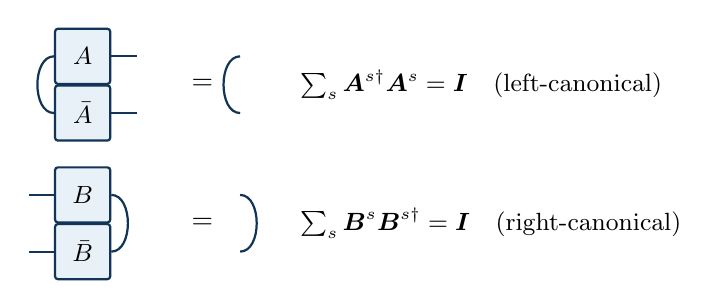
\begin{tikzpicture}[x=1cm,y=1cm]
    % --- left-canonical
    \node[tens] (A)  at (1.2, 1.55) {$A$};
    \node[tens] (Ab) at (1.2, 0.65) {$\bar A$};
    \draw[leg] (A)--(Ab);
    \draw[leg] (A.west) to[out=180,in=180] (Ab.west);
    \draw[leg] (A.east)--++(0.4,0);
    \draw[leg] (Ab.east)--++(0.4,0);
    \node at (3.1,1.1) {$=$};
    \draw[leg] (3.7,1.55) to[out=180,in=180] (3.7,0.65);
    \node[anchor=west,font=\small] at (4.5,1.1)
      {$\sum_s\Amat{s\dagger}\Amat s=\bmat I$\quad(left-canonical)};
    % --- right-canonical
    \node[tens] (B)  at (1.2,-0.65) {$B$};
    \node[tens] (Bb) at (1.2,-1.55) {$\bar B$};
    \draw[leg] (B)--(Bb);
    \draw[leg] (B.east) to[out=0,in=0] (Bb.east);
    \draw[leg] (B.west)--++(-0.4,0);
    \draw[leg] (Bb.west)--++(-0.4,0);
    \node at (3.1,-1.1) {$=$};
    \draw[leg] (3.7,-0.65) to[out=0,in=0] (3.7,-1.55);
    \node[anchor=west,font=\small] at (4.5,-1.1)
      {$\sum_s\Bmat s\Bmat{s\dagger}=\bmat I$\quad(right-canonical)};
  \end{tikzpicture}
  \end{center}
  \begin{enumerate}
    \item Prove each rule from $\sum_s\Amat{s\dagger}\Amat s=\bmat I$ and $\sum_s\Bmat s\Bmat{s\dagger}=\bmat I$.
    \item Zip the network up from the left, one site at a time. Show that the contraction reduces to the norm of the
          final tensor --- so an MPS is normalised exactly when \emph{every} tensor, that one included, is left-isometric.
    \item What is the cost of $\braket\Phi\Psi$ for two \emph{different} MPS, where nothing collapses? Why must you contract site by site and never form the $d^L$ vector?
  \end{enumerate}
\end{frame}

\begin{frame}{Exercise 2(c): overlaps from the orthogonality centre}
  Put the state in mixed-canonical form. Everything outside the centre now collapses by 2(b).
  \begin{enumerate}
    \item \textbf{Bond centre.} Show $\braket\Psi\Psi=\|\bm\Lambda_i\|_F^2=\sum_a\sigma_a^2$, and that the entanglement entropy of that cut is $-\sum_a\sigma_a^2\ln\sigma_a^2$ --- both readable off the centre alone, with \emph{no} contraction.
    \item \textbf{Two-site centre.} With $\bm\Theta^{s_is_{i+1}}=\Amat{s_i}\bm\Lambda_i\Bmat{s_{i+1}}$, show $\braket\Psi\Psi=\|\bm\Theta\|_F^2$.
  \end{enumerate}
  \centering\small\alert{This is why the DMRG eigenproblem is an ordinary one: $\bmat G=\bmat I$ comes from exactly these two rules.}
\end{frame}

\begin{frame}{Exercise 3: how many parameters does an MPS really have?}
  An MPS with bond dimensions $\chi_0=1,\chi_1,\dots,\chi_L=1$ is built from $\sum_{i=1}^{L}d\,\chi_{i-1}\chi_i$ numbers. But the gauge freedom
  $\Amat{s}_i\to\Amat{s}_i\bmat X_i$, $\Amat{s}_{i+1}\to\bmat X_i^{-1}\Amat{s}_{i+1}$ means many of them describe the \emph{same} state.
  \begin{enumerate}
    \item At each internal bond $\bmat X_i$ is any invertible $\chi_i\times\chi_i$ matrix. How many parameters does that remove?
    \item Write down the count of \emph{independent} parameters.
    \item For the \alert{maximal generic exact ranks}, $\chi_i=\min(d^i,d^{L-i})$, evaluate it for $d=2$ and $L=2,3,4$. What do you get?
    \item Prove it in general --- and explain why the answer \emph{had} to be that, in one sentence.
    \item Now cap $\chi$ \emph{below} those generic ranks. Why is the count then strictly smaller, and what does that say about the ansatz?
  \end{enumerate}
\end{frame}

% ======================================================================
\section{Summary}
% ======================================================================

\begin{frame}{Summary of week 41}
  \small
  \begin{columns}[T]
    \column{0.48\textwidth}
    \begin{block}{Thursday: operators}
      \begin{itemize}
        \item $\bmat W$ is $D\times D$ with $d\times d$ entries; $D$ counts terms open at a cut
        \item First row $=$ start, last column $=$ finish, \alert{bulk $=$ memory}
        \item Minimal $D$ is the operator Schmidt rank --- the automaton can overcount
        \item JW strings cost no $D$, but cost locality
      \end{itemize}
    \end{block}
    \column{0.48\textwidth}
    \begin{block}{Friday: the algorithm}
      \begin{itemize}
        \item Canonical form $\Rightarrow$ $\bmat G=\bmat I$ $\Rightarrow$ ordinary eigenproblem
        \item $L,R$ are $\chi\times D\times\chi$: a cut severs three lines
        \item Cost $\bigO(L\chi^3d^2D)$ --- two free bond legs, one summed
        \item Split $\bm\Theta$, keep half, move on. SVD everywhere
        \item $\varepsilon_\chi$ is an error indicator; extrapolate with it
      \end{itemize}
    \end{block}
  \end{columns}
\end{frame}

% ======================================================================
\section{Answers to the week-40 exercises}
% ======================================================================

\begin{frame}{Answers to the week-40 exercises: 1a, the norm}
  \footnotesize
  \begin{block}{1a) The norm to second order}
    With $\hat T=\sum_{ai}\delta C_{ai}a_a^{\dagger}a_i$ and $\hat T_i^2=0$ (week 39, 2c), $e^{\hat T}=\prod_i(1+\hat T_i)=1+\hat T+\sum_{i<j}\hat T_i\hat T_j+\cdots$:
    the second-order piece is the sum of \emph{products of two different} $\hat T_i$, a $2p$-$2h$ operator. In $\braket{c'}{c'}$: $1$ (zeroth order); $\element{c}{\hat T}{c}=0$ and $\element{c}{\hat T_i\hat T_j}{c}=0$ (odd and $2p$-$2h$ against the vacuum); $\element{c}{\hat T^{\dagger}\hat T}{c}=\sum_{ai,bj}\delta C^{*}_{ai}\delta C_{bj}\braket{\Phi_i^a}{\Phi_j^b}=\sum_{ai}|\delta C_{ai}|^2$.
    The cross term $\hat T^{\dagger}\hat T_i\hat T_j$ is a $1p$-$1h$ bra against a $2p$-$2h$ ket and vanishes, so the first correction to $1+\sum|\delta C|^2$ is in fact of \emph{fourth} order, $\|\sum_{i<j}\hat T_i\hat T_j\ket c\|^2$ -- safely inside the $\bigO(\delta C^3)$ claimed.
  \end{block}
  \vspace{0.3em}
  \begin{itemize}
    \item Rule used throughout: $\element{c}{\hat O}{c}$ of a normal-ordered product with respect to $\ket c$ vanishes unless the product is empty -- a quasi-particle creator anywhere kills the vacuum expectation value.
    \item The same expansion, continued to the energy, is what produces the three blocks of $\hat M$ in 1e.
  \end{itemize}
\end{frame}

\begin{frame}{Answers to the week-40 exercises: 1b, the one-body part}
  \footnotesize
  \begin{block}{1b) $\element{c}{\nc{a_i^{\dagger}a_a}\,\hat F_N\,\nc{a_b^{\dagger}a_j}}{c}$: two patterns}
    Number the operators $a_i^{\dagger}(1)\,a_a(2)\;a_p^{\dagger}(3)\,a_q(4)\;a_b^{\dagger}(5)\,a_j(6)$, with $\hat F_N=\sum_{pq}f_{pq}\nc{a_p^{\dagger}a_q}$. Pairs inside one $\nc{\ }$ are never contracted, and a non-zero contraction needs a particle pair $a_\alpha a_\beta^{\dagger}$ ($\alpha,\beta>F$) or a hole pair $a_\alpha^{\dagger}a_\beta$ ($\alpha,\beta\le F$), the first factor to the left. That leaves exactly two complete patterns:
    \begin{center}
    \begin{tabular}{@{}llll@{}}\toprule
      pattern & contractions & crossings & value\\\midrule
      I  & $(2,3)\,(4,5)\,(1,6)$: $\delta_{ap}\,\delta_{qb}\,\delta_{ij}$ & $0$, sign $+$ & $+f_{ab}\,\delta_{ij}$\\
      II & $(1,4)\,(2,5)\,(3,6)$: $\delta_{iq}\,\delta_{ab}\,\delta_{pj}$ & $3$, sign $-$ & $-f_{ji}\,\delta_{ab}$\\\bottomrule
    \end{tabular}
    \end{center}
    Sum: $f_{ab}\delta_{ij}-f_{ji}\delta_{ab}$. In the Hartree-Fock basis $f_{pq}=\varepsilon_p\delta_{pq}$, so this is $(\varepsilon_a-\varepsilon_i)\delta_{ab}\delta_{ij}=\Delta_{ai,bj}$: the one-body part of the stability matrix is the diagonal of particle-hole energies, exactly as in week 39.
  \end{block}
\end{frame}

\begin{frame}{Answers to the week-40 exercises: 1c, the particle-hole interaction}
  \footnotesize
  \begin{block}{1c) $\element{c}{\nc{a_i^{\dagger}a_a}\,\hat V_N\,\nc{a_b^{\dagger}a_j}}{c}=A_{ai,bj}$}
    $\hat V_N=\frac14\sum_{pqrs}\element{pq}{\hat v}{rs}_{\mathrm{AS}}\nc{a_p^{\dagger}a_q^{\dagger}a_sa_r}$; number $a_i^{\dagger}(1)\,a_a(2)\;a_p^{\dagger}(3)\,a_q^{\dagger}(4)\,a_s(5)\,a_r(6)\;a_b^{\dagger}(7)\,a_j(8)$.
    $a_a$ must meet $a_p^{\dagger}$ or $a_q^{\dagger}$, $a_b^{\dagger}$ must meet $a_s$ or $a_r$, $a_i^{\dagger}$ the other of $a_s,a_r$, $a_j$ the other of $a_p^{\dagger},a_q^{\dagger}$: $2\times2=4$ patterns. Pattern $(2,3)(4,8)(1,5)(6,7)$, i.e.\ $p=a$, $q=j$, $s=i$, $r=b$: the only crossing is $(1,5)$ with $(4,8)$, sign $-$, value $-\frac14\element{aj}{\hat v}{bi}_{\mathrm{AS}}$. Swapping $r\leftrightarrow s$ adds one crossing \emph{and} one antisymmetry sign; swapping $p\leftrightarrow q$ likewise. All four patterns are equal, and
    \[
      A_{ai,bj}=4\times\bigl(-\tfrac14\element{aj}{\hat v}{bi}_{\mathrm{AS}}\bigr)=-\element{aj}{\hat v}{bi}_{\mathrm{AS}}=\element{aj}{\hat v}{ib}_{\mathrm{AS}}.
    \]
    The same number is $\element{\Phi_i^a}{\hat V_N}{\Phi_j^b}$, the matrix the Tamm-Dancoff approximation diagonalises (chapter 7).
  \end{block}
  \vspace{0.3em}
  \begin{itemize}
    \item Sign rule: $(-1)^{\text{number of crossings}}$ of the contraction lines, with every line drawn above the operators; the two swaps each change the count by one \emph{and} the matrix element by a sign, which is why all four patterns agree.
    \item $A$ is the \emph{exchange-like} coupling of one particle-hole pair to another; it is what distinguishes TDA from a sum of independent excitations.
  \end{itemize}
\end{frame}

\begin{frame}{Answers to the week-40 exercises: 1d, the pair-creation part}
  \footnotesize
  \begin{block}{1d) $\element{c}{\hat V_N\,a_a^{\dagger}a_ia_b^{\dagger}a_j}{c}=B^{*}_{ai,bj}$}
    Number $a_p^{\dagger}(1)\,a_q^{\dagger}(2)\,a_s(3)\,a_r(4)\;a_a^{\dagger}(5)\,a_i(6)\,a_b^{\dagger}(7)\,a_j(8)$. Contractions among $(5)$--$(8)$ vanish ($a$ against $i$ is neither a particle nor a hole pair), so $a_s,a_r$ pair with $a_a^{\dagger},a_b^{\dagger}$ and $a_p^{\dagger},a_q^{\dagger}$ with $a_i,a_j$: four patterns again. Pattern $(3,5)(4,7)(1,6)(2,8)$, $s=a$, $r=b$, $p=i$, $q=j$: crossings $(3,5)\times(4,7)$, $(4,7)\times(1,6)$, $(1,6)\times(2,8)$ -- three, sign $-$, value $-\frac14\element{ij}{\hat v}{ba}=+\frac14\element{ij}{\hat v}{ab}_{\mathrm{AS}}$; all four agree, total $\element{ij}{\hat v}{ab}_{\mathrm{AS}}=\element{ab}{\hat v}{ij}^{*}_{\mathrm{AS}}=B^{*}_{ai,bj}$.
    Check without Wick: $a_a^{\dagger}a_ia_b^{\dagger}a_j\ket c=a_a^{\dagger}a_b^{\dagger}a_ja_i\ket c=\ket{\Phi_{ij}^{ab}}$, and $\element{c}{\hat V_N}{\Phi_{ij}^{ab}}=\element{ij}{\hat v}{ab}_{\mathrm{AS}}$ is the Condon-Slater rule. $E_0$ gives $E_0\braket{c}{\Phi_{ij}^{ab}}=0$; $\hat F_N$, a one-body operator, cannot bridge a double excitation. Pauli: $a_a^{\dagger}a_a^{\dagger}=0$ and $a_ia_i=0$, so the element vanishes unless $a\ne b$ and $i\ne j$ -- which is also what the antisymmetry of $\element{ij}{\hat v}{ab}_{\mathrm{AS}}$ says.
  \end{block}
\end{frame}

\begin{frame}{Answers to the week-40 exercises: 1e, assembling the stability matrix}
  \footnotesize
  \begin{block}{1e) $\Delta E=\frac12\bra\chi\hat M\ket\chi$}
    Expand $E=\element{c'}{\hat H}{c'}/\braket{c'}{c'}$ to second order with $e^{\hat T}=1+\hat T+\frac12\hat T^2+\cdots$ and $\hat H=E_0+\hat F_N+\hat V_N$:
    \[
      \element{c'}{\hat H}{c'}=E_0\Bigl(1+\sum|\delta C|^2\Bigr)
      +\sum\delta C^{*}_{ai}\delta C_{bj}\,(\Delta+A)_{ai,bj}
      +\tfrac12\sum\delta C_{ai}\delta C_{bj}\,B^{*}_{ai,bj}
      +\tfrac12\sum\delta C^{*}_{ai}\delta C^{*}_{bj}\,B_{ai,bj}+\bigO(\delta C^3),
    \]
    the middle term from (b) and (c), the last two from (d) and its conjugate ($\frac12\hat T^2$ carries the $\frac12$). Dividing by the norm of (a) and subtracting $E_0$ leaves
    \[
      \Delta E=\tfrac12\begin{pmatrix}\delta C^{*}&\delta C\end{pmatrix}
      \begin{pmatrix}\Delta+A&B\\B^{*}&(\Delta+A)^{*}\end{pmatrix}
      \begin{pmatrix}\delta C\\\delta C^{*}\end{pmatrix}
      =\tfrac12\bra\chi\hat M\ket\chi .
    \]
    Hermitian: $(\Delta+A)_{bj,ai}=\element{bi}{\hat v}{ja}=\element{aj}{\hat v}{ib}^{*}=(\Delta+A)^{*}_{ai,bj}$ and $B_{bj,ai}=\element{ba}{\hat v}{ji}=B_{ai,bj}$, so $B^{T}=B$, the lower-left block is $B^{*}=B^{\dagger}$, and $\hat M^{\dagger}=\hat M$.
  \end{block}
\end{frame}

\begin{frame}{Answers to the week-40 exercises: 1e, one pair, and what the diagonal means}
  \footnotesize
  \begin{block}{One pair}
    Keep a single $(a,i)$. Then $B_{ai,ai}=\element{aa}{\hat v}{ii}_{\mathrm{AS}}=0$ by antisymmetry, $\hat M=\mathrm{diag}(\Delta+A,\Delta+A)$ and
    \[
      \Delta E=|\delta C_{ai}|^2\bigl(\varepsilon_a-\varepsilon_i+A_{ai,ai}\bigr)
      =|\delta C_{ai}|^2\bigl(\varepsilon_a-\varepsilon_i-\element{ai}{\hat v}{ai}_{\mathrm{AS}}\bigr),
    \]
    since $A_{ai,ai}=\element{ai}{\hat v}{ia}=-\element{ai}{\hat v}{ai}$. This is the curvature $\element{\Phi_i^a}{\hat H}{\Phi_i^a}-E_0$ of the parabola of week 39 (and of week-39 answer 1d): the diagonal of the stability matrix is the energy of a single particle-hole excitation \emph{including} its interaction with the hole it left behind.
  \end{block}
\end{frame}

\begin{frame}{Answers to the week-40 exercises: 2a--b, what ``positive semidefinite'' means}
  \footnotesize
  \begin{block}{2a) Three statements, and which one is ``stable in every direction''}
    Spectral theorem: $\hat M=\sum_k\lambda_k\ketbra{k}{k}$ with orthonormal $\ket k$, so $\bra\chi\hat M\ket\chi=\sum_k\lambda_k|\braket{k}{\chi}|^2$. All $\lambda_k\ge0$ makes this $\ge0$; conversely $\chi=\ket k$ gives $\lambda_k\ge0$. If $\hat M=\bm C^{\dagger}\bm C$ then $\bra\chi\hat M\ket\chi=\|\bm C\chi\|^2\ge0$ (and conversely $\bm C=\hat M^{1/2}$ works). ``$\Delta E\ge0$ in every direction'' is the quadratic-form statement, $\frac12\bra\chi\hat M\ket\chi\ge0$ for every $\chi=(\delta C,\delta C^{*})$. Those $\chi$ are not all vectors -- but the block structure of $\hat M$ means that if $(u,v)$ is an eigenvector with eigenvalue $\lambda$ so is $(v^{*},u^{*})$, and their sum has the form $(\delta C,\delta C^{*})$; so the smallest value of the form on physical directions is $\lambda_{\min}(\hat M)$, and the two statements agree.
  \end{block}
  \begin{block}{2b) Why leading minors are not enough, and the hierarchy of necessary conditions}
    $\mathrm{diag}(0,-1)$: leading minors $M_{11}=0$ and $\det=0$, both $\ge0$; eigenvalue $-1$. The \emph{non-leading} principal minor $M_{22}=-1$ exposes it -- Sylvester's test with $\ge$ fails because a zero on the diagonal hides whatever follows. Restricting $\chi$ to $(\delta C,0)$ gives $\bra\chi\hat M\ket\chi=\delta C^{\dagger}(\Delta+A)\delta C$: $\Delta+A$ is the principal submatrix of $\hat M$ on the first half of the indices, and a principal submatrix of a positive semidefinite matrix is positive semidefinite (take $\chi$ supported on those indices). Necessary; not sufficient, since a general $\chi$ also feels $B$. The diagonal condition $\varepsilon_a-\varepsilon_i+A_{ai,ai}\ge0$ is the $1\times1$ principal submatrices of $\Delta+A$: weaker again -- $\begin{psmallmatrix}1&2\\2&1\end{psmallmatrix}$ has a positive diagonal and eigenvalue $-1$.
  \end{block}
\end{frame}

\begin{frame}{Answers to the week-40 exercises: 2c, the Lipkin conditions one by one}
  \footnotesize
  \begin{block}{2c) Lipkin, $N=2$, $W=0$: the conditions, one by one}
    Order the components $(\delta C_1,\delta C_2,\delta C_1^{*},\delta C_2^{*})$:
    \[
      \hat M=\begin{pmatrix}\varepsilon&0&0&V\\0&\varepsilon&V&0\\0&V&\varepsilon&0\\V&0&0&\varepsilon\end{pmatrix},
      \qquad \text{eigenvalues } \varepsilon\pm V,\ \text{each twice.}
    \]
    Diagonal: $\varepsilon>0$, always. Trace: $4\varepsilon>0$, always. $2\times2$ principal minors: $\varepsilon^2$ within a block, and $\varepsilon^2-V^2$ for the pairs $(1,4)$ and $(2,3)$ -- \alert{the first to fail}, at $|V|=\varepsilon$. $3\times3$: $\varepsilon(\varepsilon^2-V^2)$, fails at the same point. Determinant: $(\varepsilon^2-V^2)^2\ge0$ \emph{always} -- the two negative eigenvalues beyond $|V|=\varepsilon$ multiply to a positive number, so $\det\ge0$ never notices. Sylvester's \emph{leading} minors $\varepsilon,\varepsilon^2,\varepsilon(\varepsilon^2-V^2),(\varepsilon^2-V^2)^2$: the third fails. All of this is $\lambda_{\min}=\varepsilon-|V|=\varepsilon(1-\chi)$ with $\chi=|V|(N-1)/\varepsilon=|V|/\varepsilon$: the Hartree-Fock reference becomes unstable exactly at $\chi=1$, where week 39 found the deformed solution taking over.
  \end{block}
\end{frame}

\begin{frame}{Answers to the week-40 exercises: 2d, the pairing block}
  \footnotesize
  \begin{block}{2d) Pairing: $\begin{psmallmatrix}\Delta&-g/2\\-g/2&\Delta\end{psmallmatrix}$, $\Delta=\varepsilon_q-\varepsilon_p+g/2$}
    Minor: $\Delta^2-g^2/4=(\Delta-\tfrac g2)(\Delta+\tfrac g2)=(\varepsilon_q-\varepsilon_p)(\varepsilon_q-\varepsilon_p+g)\ge0$ for $g\ge0$. Eigenvalues $\Delta\mp g/2$: $\varepsilon_q-\varepsilon_p$ on $(1,1)/\sqrt2$ and $\varepsilon_q-\varepsilon_p+g$ on $(1,-1)/\sqrt2$. The lower eigenvector has $\delta C_{q\uparrow,p\uparrow}=\delta C^{*}_{q\downarrow,p\downarrow}$: both members of the pair move \emph{together}, the state stays in seniority zero, and the diagonal pairing energy of a seniority-zero determinant, $-\frac g2\times$(number of pairs), does not depend on \emph{which} levels the pairs sit on -- so the interaction cancels and only the level spacing is paid. Breaking a pair coherently costs nothing at the mean-field level beyond $\varepsilon_q-\varepsilon_p$: the determinant is stable for every $g$, and the pairing correlation (pair scattering, a $2p$-$2h$ effect) is invisible to it. Hence BCS in chapter 7, and the bond dimension of this week.
  \end{block}
\end{frame}

\begin{frame}{Answers to the week-40 exercises: 2e, when $\Delta+A$ itself fails}
  \footnotesize
  \begin{block}{2e) A negative eigenvalue of $\Delta+A$}
    $\Delta+A$ is the matrix of $\hat H-E_0$ in the space of single excitations $\ket{\Phi_i^a}$ -- the Tamm-Dancoff (CIS) matrix of chapter 7. Its eigenvector $u$ with $\lambda<0$ is a $1p$-$1h$ state $\sum_{ai}u_{ai}\ket{\Phi_i^a}$ whose energy lies \alert{below the reference}: a CIS calculation on this $\ket c$ returns a negative ``excitation energy''. On the manifold, take $\delta C=e^{i\varphi}u$ with $\varphi$ chosen so that $\mathrm{Re}\,(e^{2i\varphi}u^{T}B^{*}u)\le0$; then $\Delta E\le\lambda\|u\|^2<0$, so $\hat M\not\ge0$ whatever $B$ is.
  \end{block}
  \begin{block}{Why this is the worse case}
    \begin{itemize}
      \item When only $B$ breaks stability, $\Delta+A\ge0$: every single excitation costs energy, CIS/TDA is healthy, and the trouble shows up only in the RPA, whose frequencies $\omega^2$ turn negative -- the instability lives in the \emph{coupling} of excitation to de-excitation, i.e.\ in ground-state correlations (the Lipkin case above: $A=0$, all of it in $B$).
      \item When $\Delta+A$ fails, the reference is not even the lowest state of the space of single excitations: a \emph{single} orbital rotation lowers the energy, the Hartree-Fock iteration has converged to a saddle, and both TDA and RPA on it are meaningless. The cure is to follow $u$ downhill to the deformed determinant, as for Lipkin at $\chi>1$ -- after which a new $\hat M$ must be checked.
      \item Thouless' theorem on the RPA (chapter 7): the RPA equations have real frequencies if and only if $\hat M\ge0$. The two cases are therefore ``RPA complains'' versus ``even TDA complains''.
    \end{itemize}
  \end{block}
\end{frame}

\begin{frame}[shrink=3]{Next week, and a closing remark}
  \begin{exampleblock}{Week 42, October 15--16: back to the mean field -- the electron gas, and density functional theory}
    \small
    \textbf{Thursday:} the infinite homogeneous electron gas in Hartree-Fock (chapter 6, section 6.14): plane waves are the self-consistent orbitals, the direct term cancels against the background, the exchange energy in closed form, the single-particle energies and their logarithmic singularity at $k_F$, the energy per particle in $r_s$ and the Wigner-Seitz radius.\\
    \textbf{Friday:} density functional theory, part I (chapter 8): the electronic Hamiltonian and reduced density matrices, the Hohenberg-Kohn theorems and what they do not give, and a first functional built from the electron gas of Thursday; week 43 continues with Kohn-Sham and the local density approximation.\\
    Reading: chapter 6, section 6.14; chapter 8, sections 8.1--8.4; Szabo-Ostlund, chapter 3 for the plane-wave Hartree-Fock. \alert{No exercise sessions in weeks 42 and 43: the time is for the first midterm.} Worked answers to this week's exercises 1--3 are in the lecture notes, chapter 11, exercises 1 and 7.
  \end{exampleblock}
  \vspace{0.5em}
  \small
  Two weeks of tensor networks gave us a method with no reference determinant at all: the SVD at every bond, an automaton for the Hamiltonian, a sweep of small eigenproblems with an error read off the discarded weight. Next week we return to the determinant -- and to the one system where Hartree-Fock is solved by hand.
  \vspace{0.4em}

  \centering\alert{From entanglement back to the mean field: the electron gas, and the density as the variable.}
\end{frame}

\end{document}
